\documentclass[10pt,landscape,a4paper]{article}
\usepackage{multicol}
\usepackage{calc}
\usepackage{ifthen}
\usepackage[landscape]{geometry}
\usepackage{amssymb}
\usepackage{amsmath}
\usepackage{galois}
\usepackage{graphicx}
\usepackage{tikz}
\usetikzlibrary{matrix}

\newcommand{\invgalois}[2]{\reflectbox{\ensuremath{\galois{\reflectbox{\ensuremath{#1}}}{\reflectbox{\ensuremath{#2}}}}}}


% To make this come out properly in landscape mode, do one of the following
% 1.
%  pdflatex latexsheet.tex
%
% 2.
%  latex latexsheet.tex
%  dvips -P pdf  -t landscape latexsheet.dvi
%  ps2pdf latexsheet.ps


% If you're reading this, be prepared for confusion.  Making this was
% a learning experience for me, and it shows.  Much of the placement
% was hacked in; if you make it better, let me know...


% 2008-04
% Changed page margin code to use the geometry package. Also added code for
% conditional page margins, depending on paper size. Thanks to Uwe Ziegenhagen
% for the suggestions.

% 2006-08
% Made changes based on suggestions from Gene Cooperman. <gene at ccs.neu.edu>


% To Do:
% \listoffigures \listoftables
% \setcounter{secnumdepth}{0}


% This sets page margins to .5 inch if using letter paper, and to 1cm
% if using A4 paper. (This probably isn't strictly necessary.)
% If using another size paper, use default 1cm margins.
\ifthenelse{\lengthtest { \paperwidth = 11in}}
	{ \geometry{top=1cm,left=1cm,right=1cm,bottom=1cm} }
	{\ifthenelse{ \lengthtest{ \paperwidth = 297mm}}
		{\geometry{top=1cm,left=1cm,right=1cm,bottom=1cm} }
		{\geometry{top=1cm,left=1cm,right=1cm,bottom=1cm} }
	}

% Turn off header and footer
\pagestyle{empty}
 

% Redefine section commands to use less space
\makeatletter
\renewcommand{\section}{\@startsection{section}{1}{0mm}%
                                {-1ex plus -.5ex minus -.2ex}%
                                {0.5ex plus .2ex}%x
                                {\normalfont\large\bfseries}}
\renewcommand{\subsection}{\@startsection{subsection}{2}{0mm}%
                                {-1explus -.5ex minus -.2ex}%
                                {0.5ex plus .2ex}%
                                {\normalfont\normalsize\bfseries}}
\renewcommand{\subsubsection}{\@startsection{subsubsection}{3}{0mm}%
                                {-1ex plus -.5ex minus -.2ex}%
                                {1ex plus .2ex}%
                                {\normalfont\small\bfseries}}
\makeatother

% Define BibTeX command
\def\BibTeX{{\rm B\kern-.05em{\sc i\kern-.025em b}\kern-.08em
    T\kern-.1667em\lower.7ex\hbox{E}\kern-.125emX}}

% Don't print section numbers
\setcounter{secnumdepth}{0}


\setlength{\parindent}{0pt}
\setlength{\parskip}{0pt plus 0.5ex}


% -----------------------------------------------------------------------

\begin{document}

\raggedright
\footnotesize
\begin{multicols}{3}


% multicol parameters
% These lengths are set only within the two main columns
%\setlength{\columnseprule}{0.25pt}
\setlength{\premulticols}{1pt}
\setlength{\postmulticols}{1pt}
\setlength{\multicolsep}{1pt}
\setlength{\columnsep}{2pt}

\begin{center}
  \Large{Category Theory and Lambda-calculi} \\
% \normalsize{Basic Category Theory for Computer Scientists}\\
  \vspace{0.3cm}
  \tiny {Inspir\'{e} des notes de cours du MPRI de Paul-Andr\'{e} Melli\`{e}s, CNRS/ENS Ulm}\\
\end{center}

\section{Categories}

\textbf{Definition.} A \textbf{category} $\mathcal C$ comprises
\begin{enumerate}\setlength{\itemsep}{-0.7mm}
\item a collection of objects
\item a set $\mathsf{Hom} (A, B)$ of arrows (morphisms) $f : A \rightarrow B$ for every pair of objects $(A, B)$
\item a associative composition law $\circ : \mathsf{Hom} (B, C) \times \mathsf{Hom} (A, B) \rightarrow \mathsf{Hom} (A, C)$
\item a neutral element identity morphism $\mathsf{id}_A : A \rightarrow A$ for every object $A$
\end{enumerate}

\textbf{Example.} Category $\mathsf{Set}$
\begin{itemize}\setlength{\itemsep}{-0.7mm}
\item objects : sets
\item arrows : total functions between sets
\item composition : set-theoretic function composition
\item identities : identity functions
\end{itemize}

\textbf{Definition.} \textbf{Partial ordering} $\leq_P$ on set $P$ is a reflexive, transitive, antisymmetric relation

\textbf{Definition.} Function $f : (P, \leq_P) \rightarrow (Q, \leq_Q)$ is \textbf{order-preserving} (or \textbf{monotone}) if $p \leq_P p'$ then $f(p) \leq_Q f(p')$

\textbf{Example.} Category $\mathsf{Poset}$
\begin{itemize}\setlength{\itemsep}{-0.7mm}
\item objects : partially-ordered sets
\item arrows : order-preserving total functions
\item composition : set-theoretic function composition
\item identities : identity functions
\end{itemize}

\textbf{Remark.} Generalization of universal algebra which studies the common properties of algebraic structures.

\begin{tabular}{|c|c|c|}
  \hline
  \textbf{Category} & \textbf{Objects} & \textbf{Arrows} \\ \hline \hline
  $\mathsf{Set}$        & sets                             & total functions \\ 
  $\mathsf{Pfn}$        & sets                             & partial functions\\
  $\mathsf{FinSet}$     & finite sets                      & finite total functions\\
  $\mathsf{Mon}$        & monoids                          & monoid morphisms\\
  $\mathsf{Poset}$      & posets                           & monotone functions\\
  $\mathsf{Grp}$        & groups                           & group morphisms\\
  $\Omega\text{-}\mathsf{Alg}$ & algebras with sig $\Omega$       & $\Omega$-morphisms\\
  $\mathsf{CPO}$        & complete partial orders          & continuous functions\\
  $\mathsf{Vect}$       & vector spaces                    & linear tranforms\\
  $\mathsf{Met}$        & metric spaces                    & contraction maps\\
  $\mathsf{Top}$        & topological spaces               & continuous functions\\ \hline
\end{tabular}

\textbf{Example.} Finite categories
\begin{itemize}\setlength{\itemsep}{-0.7mm}
\item category $0$ : no objects, no arrows
\item category $1$ : one object, one arrow
\item category $2$ : two objects, two identity arrows, arrow from one object to another
\item category $3$ : objects $A$, $B$, $C$, three identity arrows, three arrows $f : A \rightarrow B$, $g : B \rightarrow C$, $h : A \rightarrow C$
\end{itemize}

\textbf{Remark.} Categorical logic : objects as arbitrary category formulas, arrows $f : A \rightarrow B$ as proofs of $A \Rightarrow B$. Identity $\mathsf{id}_A$ is an instance of reflexivity and following inference rule asserts transitivity of $\Rightarrow$
\vspace{-0.1cm}
\begin{eqnarray*}
\frac{f : A \rightarrow B \quad \quad g : B \rightarrow C}{g \circ f : A \rightarrow C}
\end{eqnarray*}

\textbf{Definition.} $\mathcal C^{\text{op}}$ is \textbf{dual category} of $\mathcal C$ if it  has same objects and opposite arrows of $\mathcal C$

\textbf{Definition.} $\mathcal C \times \mathcal D$ is \textbf{product category} of $\mathcal C$ and $\mathcal D$ if it has objects pairs $(A, B)$, arrow pairs $(f, g)$. Pairwise defined composition and identity arrows.

\section{Diagrams}

\textbf{Definition.} \textbf{Diagram in} $\mathcal C$ is a collection of vertices and directed edges, consistently labeled with objects and arrows of $\mathcal C$.

\textbf{Definition.} Diagram in $\mathcal C$ \textbf{commutes} if, for every pair of vertices $X$ and $Y$, all the paths in the diagram from $X$ to $Y$ are equal

% rajouter l'exemple page 11
% et morphismes, produit et exponentiation de catégories


\section{Functors}

\textbf{Definition.} A \textbf{functor} $F : \mathcal C \rightarrow \mathcal D$ comprises
\begin{enumerate}\setlength{\itemsep}{-0.7mm}
\item for every $A$ of $\mathcal C$, an object $FA$ of $\mathcal D$
\item for every pair $(A, B)$ of objects of $\mathcal C$, a function $F_{A, B} : \mathsf{Hom}_{\mathcal {C}} (A, B) \rightarrow \mathsf{Hom}_{\mathcal {D}} (FA, FB)$
\end{enumerate}
preserving
\begin{enumerate}\setlength{\itemsep}{-0.7mm}
\item composition : $FA \overset{F f}{\longrightarrow} FB \overset{F g}{\longrightarrow} FC \quad = \quad FA \overset{F (g \circ f)}{\longrightarrow} FC$
\item identities : $FA \overset{F \mathsf{id}_{A}}{\longrightarrow} FA \quad = \quad FA \overset{\mathsf{id}_{FA}}{\longrightarrow} FA$
\end{enumerate}

\section{Natural transformations}

\textbf{Definition.} A \textbf{natural transformation} $\theta : F \Rightarrow G$ from functors $F$ to $G$ (both from $\mathcal C$ to $\mathcal D$) is a family of morphisms $\Big (\theta_A ~:~ FA \rightarrow GA \Big )_{A \in \mathsf{Obj} (\mathcal{C})}$ such that for all $\mathcal C$-arrow $f : A \rightarrow B$, commutes in $\mathcal D$
\vspace{-0.3cm}
\begin{center}
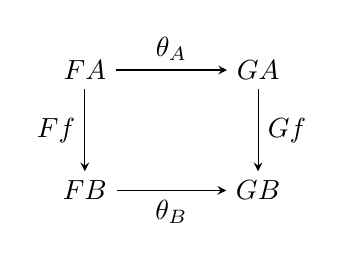
\begin{tikzpicture}
  \matrix (m) [matrix of math nodes,row sep=3em,column sep=4em,minimum width=2em] {
     FA & GA \\
     FB & GB \\};
  \path[-stealth]
    (m-1-1) edge node [left] {$F f$} (m-2-1)
            edge node [above] {$\theta_A$} (m-1-2)
    (m-2-1.east|-m-2-2) edge node [below] {$\theta_B$} (m-2-2)
    (m-1-2) edge node [right] {$G f$} (m-2-2);
\end{tikzpicture}
\end{center}
\vspace{-0.2cm}
% dessiner le schéma du TD de Mimram

If every $\eta_A$ of $\eta$ is an isomorphism in $\mathcal D$ then $\eta$ is a \textbf{natural isomorphism}.

\textbf{Example.} $\mathsf{rev}_S : \mathsf{List}~S \rightarrow \mathsf{List}~S$ is a natural transformation
\begin{itemize}
\item if $f : S \rightarrow T$ then $\mathsf{rev}_T \circ \mathsf{maplist}~f = \mathsf{maplist}~f \circ \mathsf{rev}_S$
\end{itemize}

\section{Adjunctions}

\textbf{Definition.} An \textbf{adjunction} $(L, R, \phi)$ comprises
\begin{enumerate}\setlength{\itemsep}{-0.7mm}
\item functors $L : \mathcal C \rightarrow \mathcal D$, $R : \mathcal D \rightarrow C$
\item a family $\phi$ of natural bijections in $\mathcal C$ and $\mathcal D$, for every $\mathcal C$-object $C$ and $\mathcal D$-object $D$, \quad
  $\mathsf{Hom}_{\mathcal{D}} (L C, D) \cong \mathsf{Hom}_{\mathcal{C}} (C, R D)$

written $\displaystyle\frac{LC \rightarrow_{\mathcal{D}} D}{C \rightarrow_{\mathcal{C}} RD} \phi_{A,B}$
\end{enumerate}

\textbf{Notation.} $L \dashv R$ : $L$ is \textbf{left adjoint to} $R$

\section{Monads}

\textbf{Definition.} A \textbf{monad} $(T, \mu, \eta)$ comprises
\begin{enumerate}\setlength{\itemsep}{-0.7mm}
\item an endofunctor $T : \mathcal C \rightarrow \mathcal C$
\item natural transformations $\mu : T \circ T \Rightarrow T$ and $\eta : \mathsf{id}_{\mathcal{C}} \Rightarrow T$ such that commutes
\end{enumerate}

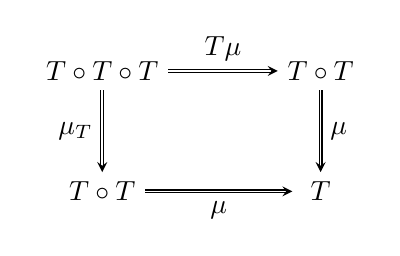
\begin{tikzpicture}
  \matrix (m) [matrix of math nodes,row sep=3em,column sep=4em,minimum width=2em] {
     T \circ T \circ T & T \circ T \\
     T \circ T         & T \\};
  \path[-stealth]
    (m-1-1) edge [double] node [left] {$\mu_T$} (m-2-1)
            edge [double] node [above] {$T \mu$} (m-1-2)
    (m-2-1.east|-m-2-2) edge [double] node [below] {$\mu$} (m-2-2)
    (m-1-2) edge [double] node [right] {$\mu$} (m-2-2);
\end{tikzpicture}%
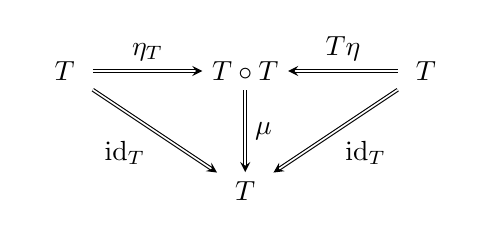
\begin{tikzpicture}
  \matrix (m) [matrix of math nodes,row sep=3em,column sep=4em,minimum width=2em] {
     T & T \circ T & T \\
       & T         & \\};
  \path[-stealth]
  (m-1-1) edge [double] node [below left] {$\text{id}_T$} (m-2-2)
  edge [double] node [above] {$\eta_T$} (m-1-2)
  (m-1-2) edge [double] node [right] {$\mu$} (m-2-2)
  (m-1-3) edge [double] node [below right] {$\text{id}_T$} (m-2-2)
  edge [double] node [above] {$T \eta$} (m-1-2)
  ;
\end{tikzpicture}

\textbf{Definition.} Every set $S$ induces the \textbf{state monad} $X ~ \mapsto ~ S \Rightarrow (S \times X) ~:~ \mathsf{Set} \rightarrow \mathsf{Set}$ by the adjunction
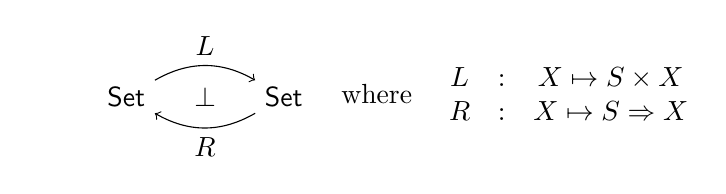
\begin{tikzpicture}
  \node [] (s1)  [] {$\mathsf{Set}$};
  \node [] (bot) [right of=s1] {$\bot$};
  \node [] (s2)  [right of=bot] {$\mathsf{Set}$};
  \node [] (text)  [right of=s2] {\quad\quad\quad\quad\quad\quad\quad\quad\quad\quad\quad where \quad $\begin{matrix}
      L &:& X \mapsto S \times X\\ 
      R &:& X \mapsto S \Rightarrow X
    \end{matrix}$};
  \path[->] 
  (s1) edge [bend left] node [above] {$L$} (s2)
  (s2) edge [bend left] node [below] {$R$} (s1);
\end{tikzpicture}

\textbf{Definition.} \textbf{Kleisli category} $\mathcal C_T$ of monad $(T, \mu, \eta)$ has
\begin{enumerate}
\item same objects as $\mathcal C$
\item morphisms $A \twoheadrightarrow B$ as morphisms $A \rightarrow TB$ in $\mathcal C$
\item identities $\mathsf{id}_A : A \twoheadrightarrow A$ given by $\eta_A : A \rightarrow T A$
\item compositions $g \circ_{\textsf{K}} f$ of $f : A \twoheadrightarrow B$, $g : B \twoheadrightarrow C$ as
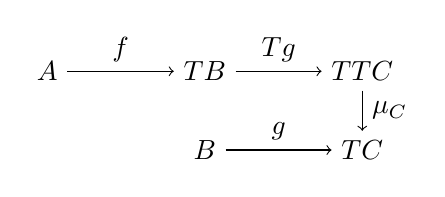
\begin{tikzpicture}
  \node [] (s1)  [] {$A$};
  \node [] (s1')  [right of=s1] {};
  \node [] (t2) [right of=s1'] {$TB$};
  \node [] (t2') [right of=t2] {};
  \node [] (u3) [right of=t2'] {$TTC$};
  \node [] (s2) [below of=t2] {$B$};
  \node [] (t3) [below of=u3] {$TC$};
  \path[->] 
  (s1) edge [] node [above] {$f$} (t2)
  (t2) edge [] node [above] {$T g$} (u3)
  (s2) edge [] node [above] {$g$} (t3)
  (u3) edge [] node [right] {$\mu_C$} (t3);
\end{tikzpicture}

\end{enumerate}

\textbf{Example.} Monads in \textsf{OCaml}
\vspace{-0.2cm}
\begin{verbatim}
Monads can be viewed as a standard programming interface
to various data or control structures, which is captured
by the 'a t type. All common monads are members of it:

(>>=)  : 'a t -> ('a -> 'b t) -> 'b t     (* bind/unit *)
return : 'a   -> 'a t
run    : 'a t -> 'a

All instances of monad should obey the following equations:

return a >>= f          = f a            (* left unit *) 
a >>= fun x -> return x = a              (* right unit *) 
(a >>= fun x -> b) >>= fun y -> c
      = a >>= fun x -> b >>= fun y -> c  (* associativity *)
\end{verbatim}


\section{Domain theory}
\textbf{Definition.} Pair of maps $X ~ \invgalois{f^R}{f} ~ Y$ is an \textbf{embedding} of $X$ into $Y$ if $f^R \circ f = \mathsf{id}_X$ and $f \circ f^R \sqsubseteq \mathsf{id}_Y$.

\textbf{Remark.} $f \sqsubseteq g$ : $f$ \emph{approximates} $g$ in some ordering representing their information content
\begin{center}
    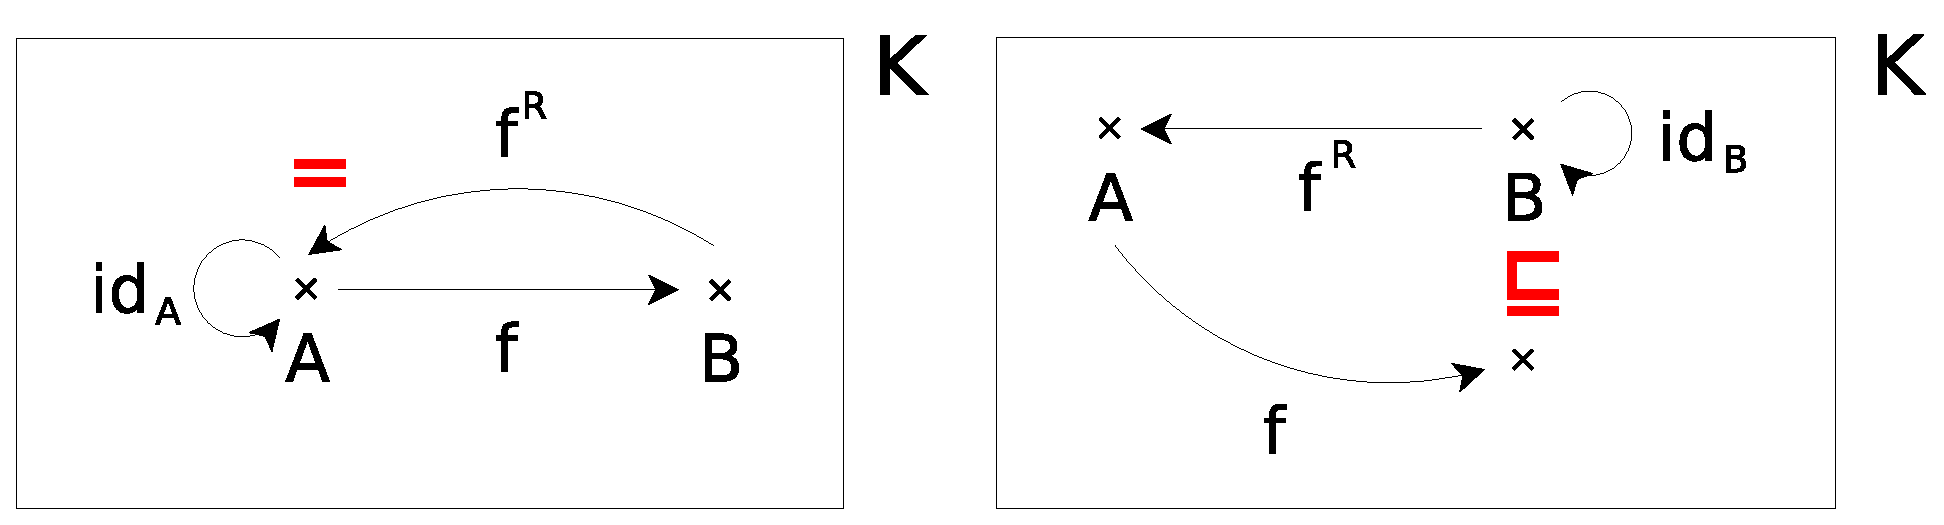
\includegraphics[width=0.3\textwidth]{figures/plongement.eps}
\end{center}

%%%%%%%%%%%%%%%%%%%%%%%%%%%%%%%%%%%%%%%%%%%%%%%%%%%%%%%%%%%%%%%%%%%%%%%%%%%%%%%%%%%%



\rule{0.3\linewidth}{0.25pt}
\scriptsize

\LaTeX \ cheat sheet template made by Winston Chang

http://www.stdout.org/$\sim$winston/latex/


\end{multicols}
\end{document}
